% Copyright 2019 by Saeed Taghavi
%
% This file may be distributed and/or modified
%
% 1. under the LaTeX Project Public License and/or
% 2. under the GNU Public License.
%
% See the file doc/licenses/LICENSE for more details.

\documentclass{beamer}

% Setup appearance:

\usetheme{Darmstadt}
\usefonttheme[onlylarge]{structurebold}
\setbeamerfont*{frametitle}{size=\normalsize,series=\bfseries}
\setbeamertemplate{navigation symbols}{}


% Standard packages

\usepackage[english]{babel}
\usepackage[latin1]{inputenc}
\usepackage{times}
\usepackage[T1]{fontenc}


% Setup TikZ

\usepackage{tikz}
\usetikzlibrary{arrows}
\tikzstyle{block}=[draw opacity=0.7,line width=1.4cm]


% Author, Title, etc.

\title[Short title] 
{%
Phase-Dependent Suppression of Neuronal Oscillations
%
}

\author[Taghavi, Valizadeh]
{
  \textcolor{blue!50!black}{Saeed~Taghavi\inst{1}} \and
  Alireza~Valizadeh\inst{1,2}
}

\institute[IASBS and others]
{
  \inst{1}%
  IASBS, Zanjan, Iran
  \and
  \vskip-2mm
  \inst{2}%
  IPM, Tehran, Iran
}

\date[neurophysics 2020]
{Conference on Neuroscience \\ and Physics of Neuronal Systems \\ 19 and 20 February 2020
\\
}





% The main document

\begin{document}

\begin{frame}
  \titlepage
\end{frame}

\begin{frame}{Outline}
  \tableofcontents
\end{frame}

%inja


\section{Introduction}

%\subsection{The Model and the Problem}
\subsection{The Problem}

\begin{frame}{Neural synchrony in brain disorders}


Certain brain disorders are associated with abnormaly neural synchronization.
%  Dysfunctional communication resulting from an inability to properly modulate oscillatory activity, either through hypo- or hyper-synchrony, has been implicated in a number of neurological disorders.
%In Parkinson's disease (PD), movement impairment is correlated with exaggerated beta frequency oscillations in the cerebral cortex and subthalamic numcleus(STN).
%There is evidence for enhanced synchronized $\beta$-band activity prior to movement preparation and during visuo-motor coordination.
\\
  \begin{block}{remember}
      Shanon entropy\\
      \begin{equation*}
        H=\Sigma_{i=1}^{N} -p_{i}\log(p_{i})
      \end{equation*}
  \end{block}
\end{frame} 

\begin{frame}[t]{General formalization of haplotyping.}
  \begin{block}{Inputs}
    \begin{itemize}
    \item A \alert{genotype matrix} $G$.
    \item The \alert{rows} of the matrix are \alert{taxa / individuals}.
    \item The \alert{columns} of the matrix are \alert{SNP sites /
        characters}. 
    \end{itemize}
  \end{block}
  \begin{block}{Outputs}
    \begin{itemize}
    \item A \alert{haplotype matrix} $H$.
    \item Pairs of rows in $H$ \alert{explain} the rows of $G$.
    \item The haplotypes in $H$ are \alert{biologically plausible}. 
    \end{itemize}
  \end{block}
\end{frame}


\begin{frame}[t]{Our formalization of haplotyping.}
  \begin{block}{Inputs}
    \begin{itemize}
    \item A genotype matrix $G$.
    \item The rows of the matrix are individuals / taxa.
    \item The columns of the matrix are SNP sites / characters.
    \item<alert@1->
      The problem is directed: one haplotype is known.
    \item<alert@1->
      The input is biallelic: there are only two homozygous
      states (0 and 1) and one heterozygous state (2).
    \end{itemize}
  \end{block}
  \begin{block}{Outputs}
    \begin{itemize}
    \item A haplotype matrix $H$.
    \item Pairs of rows in $H$ explain the rows of $G$.
    \item<alert@1> The haplotypes in $H$ form a perfect phylogeny.
    \end{itemize}
  \end{block}
\end{frame}


\begin{frame}{We can do perfect phylogeny haplotyping efficiently, but
    \dots}
  \begin{enumerate}
  \item \alert{Data may be missing.}
    \begin{itemize}
    \item This makes the problem NP-complete \dots
    \item \dots even for very restricted cases.
    \end{itemize}
    \textcolor{green!50!black}{Solutions:}
    \begin{itemize}
    \item Additional assumption like the rich data hypothesis. 
    \end{itemize}
  \item \alert{No perfect phylogeny is possible.}
    \begin{itemize}
    \item This can be caused by chromosomal crossing-over effects.
    \item This can be caused by incorrect data.
    \item This can be caused by multiple mutations at the same sites.
    \end{itemize}
    \textcolor{green!50!black}{Solutions:}
    \begin{itemize}
    \item Look for phylogenetic networks.
    \item Correct data.
    \item<alert@1->
       Find blocks where a perfect phylogeny is possible.
    \end{itemize}
  \end{enumerate}
\end{frame}


\subsection{The Integrated Approach}

\begin{frame}{How blocks help in perfect phylogeny haplotyping.}
  \begin{enumerate}
  \item Partition the site set into overlapping contiguous blocks.
  \item Compute a perfect phylogeny for each block and combine them.
  \item Use dynamic programming for finding the partition.
  \end{enumerate}

  \begin{tikzpicture}
    \useasboundingbox (0,-1) rectangle (10,2);
    
    \draw[line width=2mm,dash pattern=on 1mm off 1mm]
      (0,1) -- (9.99,1) node[midway,above] {Genotype matrix}
      (0,0.6666) -- (9.99,0.6666)
      (0,0.3333) -- (9.99,0.3333)
      (0,0) -- (9.99,0) node[midway,below] {\only<1>{no perfect phylogeny}};

    \begin{scope}[xshift=-.5mm]
      \only<2->
      {
        \draw[red,block]            (0,.5)   -- (3,.5)
          node[midway,below] {perfect phylogeny};
      }
        
      \only<3->
      {
        \draw[green!50!black,block] (2.5,.5)   -- (7,.5)
          node[pos=0.6,below] {perfect phylogeny};
      }

      \only<4->
      {
        \draw[blue,block]           (6.5,.5) -- (10,.5)
          node[pos=0.6,below] {perfect phylogeny};
      }
    \end{scope}
  \end{tikzpicture}
\end{frame}

\begin{frame}{Objective of the integrated approach.}
  \begin{enumerate}
  \item Partition the site set into \alert{noncontiguous} blocks. 
  \item Compute a perfect phylogeny for each block and combine them. 
  \item<alert@1-> Compute partition while computing perfect
    phylogenies. 
  \end{enumerate}

  \begin{tikzpicture}
    \useasboundingbox (0,-1) rectangle (10,2);

    \draw[line width=2mm,dash pattern=on 1mm off 1mm]
      (0,1) -- (9.99,1) node[midway,above] {Genotype matrix}
      (0,0.6666) -- (9.99,0.6666)
      (0,0.3333) -- (9.99,0.3333)
      (0,0) -- (9.99,0) node[midway,below] {\only<1>{no perfect phylogeny}};

    \only<2->
    {
      \begin{scope}[xshift=-0.5mm]
        \draw[red,block] (0,.5)   -- (3,.5) 
          node[midway,below] {perfect phylogeny}
                         (8,.5) -- (9,.5);

        \draw[green!50!black,block]
          (3,.5)   -- (6,.5)
            node[pos=0.6,below] {perfect phylogeny}
          (6.4,.5)   -- (8,.5)
          (9,.5) -- (10,.5);

        \draw[blue,block] (6,.5) -- (6.4,.5)
          node[midway,below=5mm] {perfect phylogeny};
      \end{scope}
    }
  \end{tikzpicture}
\end{frame}


\begin{frame}{The formal computational problem.}
  We are interested in the computational complexity of \\
  \alert{the function \alert{$\chi_{\operatorname{PP}}$}}:
  \begin{itemize}
  \item It gets genotype matrices as input.
  \item It maps them to a number $k$.
  \item This number is minimal such that the sites can be
    covered by $k$ sets, each admitting a perfect phylogeny.
    \\
    (We call this a \alert{pp-partition}.)
  \end{itemize}
\end{frame}


\subsection{Phase Response Curve}
\begin{frame}{The Phase Response Curve (PRC)}
  We are interested in the computational complexity of \\
  \alert{the function \alert{$\chi_{\operatorname{PP}}$}}:
  \begin{itemize}
  \item It gets genotype matrices as input.
  \item It maps them to a number $k$.
  \item This number is minimal such that the sites can be
    covered by $k$ sets, each admitting a perfect phylogeny.
    \\
    (We call this a \alert{pp-partition}.)
  \end{itemize}
\end{frame}


\headerbox{Numerical results}{name=results1,column=0,below=introduction,span=3}{

\begin{multicols}{2}

\large{
To model the neuronal populations that generate pathological oscillations, we have used a network of $N=1000$ coupled oscillators . The time evolution of the set of each oscillator is given by the Kyramoto equations
\begin{center}
$ \qquad \qquad \qquad  \frac{d\theta_{i}}{dt}=\omega_i + \frac{k}{N} \Sigma_{j=1}^N \sin (\theta_j - \theta_i) + I X(t) Z(\theta_i)$
\end{center}
%$ \qquad \qquad \qquad  \frac{d\theta_{i}}{dt}=\omega_i + \frac{k}{N} \Sigma_{j=1}^N \sin (\theta_j - \theta_i) + I X(t) Z(\theta_i)$

The first term, $\omega_i$ is the natural frequency of oscillator $i$, which describes the frequency in the absence of external inputs. It corresponds to the frequency with which a neuron spontaneously produces spikes or bursts (depending of the interpretation of oscillators introduced above). The second term describes the interactions between oscillators, where $k$ is the coupling constant which controls the strength of coupling between each pair of oscillators and hence their tendency to synchronize. The third term describes the effect of stimulation. The intensity of stimulation is denoted by $I$ and $X(t)$ is a function which equals $1$ if stimulation is applied at time $t$ and $0$ otherwise. The phase response function for a single oscillator is denoted by $Z(\theta_i )$.
\\
The intensity of stimulation was chosen to be $I \approx 5$  Numerical integration was performed using Euler method with a time step of $dt \approx 0.01 $. 
\begin{center}
\includegraphics[width=0.65\linewidth]{fig/order_param1} 
\end{center}
}
\center{
%\vspace*{-.5cm}
\includegraphics[width=0.9\linewidth]{fig/theta-main} 
}
\end{multicols}

%\vspace{1.15cm}
%\vspace{2cm} %remove this, only added for spacing
}
\headerbox{Conclusion}{name=subtopic1,column=2,below=results1,span=1}{
\large{
The amplitude of collective oscillations could be modulated depending on the specific phase at which the stimulation is applied. 

Also, we could predict the $good \ time$ for applying stimulation to get the maximum reduction in the oscillation amplitude based on the phase response curve (PRC) of oscillators.
}
\\

\\

\vspace*{1.6cm}
}


\headerbox{Discussion}{name=subtopic3,column=0,below=results1,span=2}{
%\vspace{0.3cm}
\begin{multicols}{2}
\large{

\center{
%\vspace*{-.5cm}
\includegraphics[width=0.8\linewidth]{fig/deltaR-Z} 
}

\center{
%\vspace*{-.5cm}
\includegraphics[width=0.7\linewidth]{fig/multi_stim} 
}


Applying multiple stimulations 

}
\end{multicols}

%\vspace{2cm} %remove this, only added for spacing
}


\section*{Conclusion}

\begin{frame}
  \frametitle<presentation>{Summary}

  \begin{itemize}
  \item
    Finding optimal pp-partitions is \alert{intractable}. 
  \item
    It is even intractable to find a pp-partition when \alert{just two 
      noncontiguous  blocks are known to suffice}.
  \item
    For perfect \alert{path} phylogenies, optimal partitions can be
    computed \alert{in polynomial time}.
  \end{itemize}

   \uncover<2>{
     \begin{columns}[t]
    \column{.5\textwidth}
    \begin{block}{}
    \begin{center}
      Thank you for listening!
      \\
      Any Questions?
    \end{center}

    \end{block}
    \end{columns}  
%  \begin{block}{}
%  {
%  \begin{center}
%
%  
%  \end{center}
%  }
%  \end{block}   
   } 
\end{frame}



\appendix

\section*{Appendix}

\begin{frame}[label=algorithm]{The algorithm in action.}{Computation of
    the partial order.}
  \begin{columns}[t]
    \column{.4\textwidth}
    \begin{exampleblock}{Genotype matrix}
      $G\colon$
      \begin{tabular}{ccccc}
        A & B & C & D & E \\\hline
        2 & 2 & 2 & 2 & 2 \\
        0 & 1 & 2 & 1 & 0 \\
        1 & 0 & 0 & 1 & 2 \\
        0 & 2 & 2 & 0 & 0
      \end{tabular}
    \end{exampleblock}
    \column{.6\textwidth}
    \begin{exampleblock}{Partial order}
      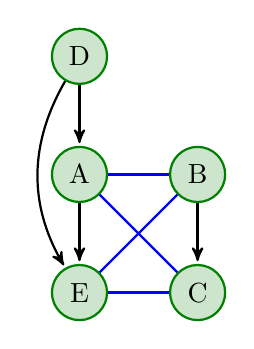
\begin{tikzpicture}[node distance=15mm]
        \tikzstyle{every node}=
        [%
          fill=green!50!black!20,%
          draw=green!50!black,%
          minimum size=7mm,%
          circle,%
          thick%
        ]

        \node (A) {A};
        \node (B) [right of=A] {B};
        \node (C) [below of=B] {C};
        \node (D) [above of=A] {D};
        \node (E) [below of=A] {E};

        \path [thick,shorten >=1pt,-stealth'] (A) edge (E)
                         (B) edge (C)
                         (D) edge (A)
                             edge[bend right] (E);

        \uncover<2>{
        \path [-,blue,thick](A) edge (B)
                                edge (C)  
                            (B) edge (E)
                            (C) edge (E);}
      \end{tikzpicture}

      Partial order: \tikz[baseline] \draw[thick,-stealth'] (0pt,.5ex)
      -- (5mm,.5ex); 

      \uncover<2>{\textcolor{blue}{Compatible as children of root:
          \tikz[baseline] \draw[thick] (0pt,.5ex) -- (5mm,.5ex);}} 
    \end{exampleblock}
  \end{columns}  
\end{frame}

\begin{frame}{The algorithm in action.}{The matching in the special graph.}
  \begin{columns}[t]
    \column{.3\textwidth}
    \begin{exampleblock}{Partial order}
      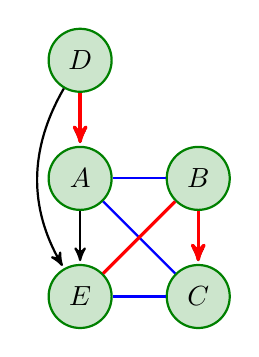
\begin{tikzpicture}[node distance=15mm]
        \tikzstyle{every node}=%
        [%
          fill=green!50!black!20,%
          draw=green!50!black,%
          minimum size=8mm,%
          circle,%
          thick%
        ]

        \node (A)              {$A$};
        \node (B) [right of=A] {$B$};
        \node (C) [below of=B] {$C$};
        \node (D) [above of=A] {$D$};
        \node (E) [below of=A] {$E$};

        \path [thick,shorten >=1pt,-stealth'] (A) edge (E)
                         (B) edge (C)
                         (D) edge (A)
                             edge[bend right] (E);

        \path [-,blue,thick](A) edge (B)
                                edge (C)  
                            (B) edge (E)
                            (C) edge (E);

        \only<3->
        {
          \path[very thick,shorten >=1pt,-stealth',red] (D) edge (A) (B) edge (C);
          \path [-,red,very thick](E) edge (B);
        }
      \end{tikzpicture}
    \end{exampleblock}
    \column{.7\textwidth}
    \begin{exampleblock}{Matching graph}
      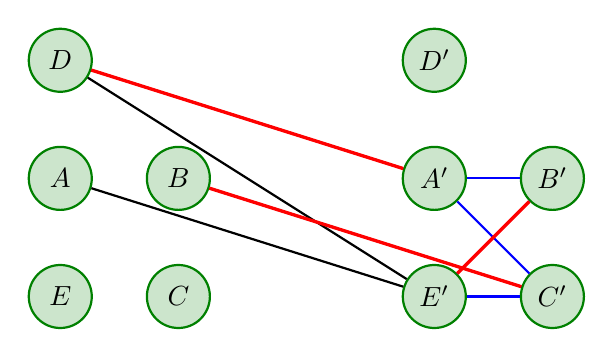
\begin{tikzpicture}[node distance=15mm]
        \tikzstyle{every node}=%
        [%
          fill=green!50!black!20,%
          draw=green!50!black,%
          minimum size=8mm,%
          circle,%
          thick,%
          inner sep=0pt%
        ]

        \node (A)              {$A$};
        \node (B) [right of=A] {$B$};
        \node (C) [below of=B] {$C$};
        \node (D) [above of=A] {$D$};
        \node (E) [below of=A] {$E$};

        \begin{scope}[xshift=4.75cm]
          \node (A')               {$A'$};
          \node (B') [right of=A'] {$B'$};
          \node (C') [below of=B'] {$C'$};
          \node (D') [above of=A'] {$D'$};
          \node (E') [below of=A'] {$E'$};
        \end{scope}
        
        \path [thick]    (A) edge (E')
                         (B) edge (C')
                         (D) edge (A')
                             edge (E');

        \path [blue,thick](A') edge (B')
                               edge (C')  
                          (B') edge (E')
                          (C') edge (E');

        \only<2->
        {
          \path[very thick,red] (D) edge (A')
                           (B) edge (C')
                           (B') edge (E');
        }
      \end{tikzpicture}
    \end{exampleblock}
  \end{columns}

  \medskip
  \uncover<2->{A \alert{maximal matching} in the matching graph
    \uncover<3>{induces\\ \alert{perfect path phylogenies}.}}

  \hfill\hyperlink{return}{\beamerreturnbutton{Return}}
\end{frame}

\end{document}


